\section*{Process description}


Nitroma's process for the nitration of toluene and subsequent reduction and hydrogenation of nitrotoluenes is unique in both its continuous operating mode and the production of three different substituted aromatic amines.  \Cref{fig:BFD-ES} is a simplified process flow diagram of the process.
\begin{wrapfigure}{l}{0.55\linewidth}
    \centering
    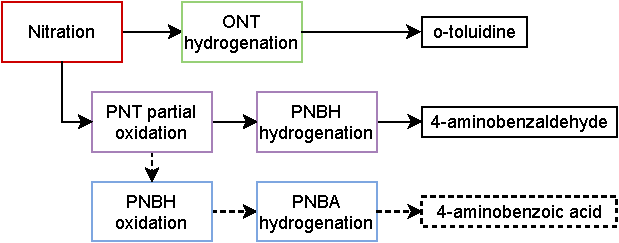
\includegraphics[width=0.8\linewidth]{chapters/0-executive-summary/figures/BFD_nitroma-Page-3.pdf}
    \caption{Simplified synthesis route for Nitroma's process}
    \label{fig:BFD-ES}
\end{wrapfigure}

Firstly, the nitration of toluene with 70\% aqueous nitric acid is carried out in a shell-and-tube heat exchanger reactor packed with H-mordenite catalyst. Solid acid catalysts were preferred over the traditional mixed-acid synthesis due to environmental, safety and performance advantages. Zeolites indeed alleviate the need for costly and energy intensive regeneration of corrosive sulphuric acid, as well as preventing the emission of toxic and global warming potential nitrogen oxides. Heterogeneous catalysis is also attractive from an economical point of view since it favours the more economically desirable \para-nitrotoluene (PNT) isomer. The nitration reactor effluent is fed to a decanter to separate the aqueous nitric acid from the organic phase. Following water evaporation in a distillation column, nitric acid is recycled back into the nitration reactor at a \SI{94}{mol\percent} purity. Meanwhile, the organic phase is sent to a distillation column to recycle unreacted toluene to the nitration reactor. The nitrotoluenes are sent to a second distillation column to separate the more volatile o-nitrotoluene (ONT) from m-nitrotoluene (MNT) and PNT. The large difference in the PNT and MNT melting points is exploited in a mixed-suspension mixed-product removal crystalliser, followed by a hydraulic wash column.

Liquid ONT is mixed with methanol and hydrogenated under pressure over Pd/C catalyst to o-toluidine (o-TOL) in a co-current trickle bed reactor operating with both gas and liquid in downflow mode. Trickle bed reactor is chosen due to the ease of operation at high pressure and the relative slow catalyst deactivation, which is imperative for an expensive catalyst usage. o-TOL is then purified to achieved a purity of \SI{99.4}{mol\percent}. The hydrogen gas leaves the reactor via an outlet port, and the effluent enters a distillation column to separate methanol and water from the less volatile organic compounds. Methanol is further distilled to be recycled to the reactor. 

Meanwhile, gaseous PNT is fed into an air-oxidation reactor packed with cobalt phthalocyanine catalyst to be partially oxidised to 4-nitrobenzaldehyde (4-NBH). Depending on the production campaign, the reactor effluent can either be sent to a second oxidation reactor where 4-NBH and unreacted PNT will be completely oxidised to 4-nitrobenzoic acid (4-NBA), owing to longer resistence times; or to a liquid-phase hydrogenation reactor. 4-NBH and 4-NBA are both reduced to respectively 4-aminobenzaldehyde (4-ABH) and 4-aminobenzoic acid (4-ABA) with formic acid diluted in a methanol solvent over Pt/C catalyst. 4-ABH is purified via a sequence of distillation packed columns whereas 4-ABA is recovered as a solid following  crystallisation in a continuous falling-film melt crystalliser.







 

